\section{Finite State Machine (FSM)}

\subsection{Zustandsbasierte Systeme}

\subsubsection{Asynchron vs.synchrone FSMs}
\begin{itemize}
  \item Bei (elektronisch implementierten) asynchronen FSMs führen geänderte
  Inputsignale direkt zu Zustandsänderungen. Sie sind deshalb "`schneller"',
  jedoch äusserst empfindlich auf Glitches und kaum testbar.
  \item Bei synchronen FSMs werden die Inputsignale nur zu diskreten Zeitpunkten
  betrachtet, diese Systeme sind getaktet.
  \item Softwareimplementationen sind eigentlich immer synchron, da die Rechner
  getaktet sind. Wenn die Inputsignale mittels Interrupts behandelt werden, ist
  darauf zu achten, dass die Interrupts nicht fälschlicherweise gesetzt werden (ist Aufgabe der Elektronik)
  \item Rein softwareseitig besteht die Problematik der Asynchronizität nicht
\end{itemize}

\subsubsection{Finite State Machine (FSM)}
\begin{itemize}
  \item Eine FSM befindet sich immer in einem definierten Zustand
  \item Die Inputs X bezeichnen üblicherweise Ereignisse (Events)
  \item Die Outputs Y werden oft auch Actions genannt
  \item Eine FSM benötigt immer Speicherelemente zur Speicherung des internen Zustands
  \item In der Praxis sind zwei FSM-Varianten bekannt: \begin{itemize}
			\item der Mealy-Automat
			\item der Moore-Automat
  			\end{itemize}
\end{itemize}
  
\subsubsection{Zustands-Ereignis-Diagramm (State-Event-Diagram)}
\begin{itemize}
  \item Die Zustände werden mit einem Kreis gekennzeichnet
  \item Die Ereignisse werden mit Pfeilen zwischen den Zuständen bezeichnet
  (Transitionen)
  \item Die Aktionen werden entweder bei den Zuständen geschrieben oder bei den
  Transitionen (je nach Automatentyp)
  \item Die Ausführung einer Transition benötigt keine Zeit. Deshalb sind bei
  der Modellierung oft Zwischenzustände vorzusehen, z.B. "`Closing"', "`Starting
  up"', "`Booting"', etc.
\end{itemize}

\subsubsection{Mealy-Automat}
\begin{itemize}
  	\item Der nächste Zustand $Z_{n+1}$ ist abhängig vom Input X und von $Z_n$:
  	$Z_{n+1}=f(Z_n,X)$
  	\item Der Output Y ist abhängig vom inneren Zustand $Z_n$ \textbf{und vom
 	 Input X}: $Y=g(Z_n, X)$
  	\item Die Actions liegen deshalb bei den Transitionen
\end{itemize}

\subsubsection{Moore-Automat}
\begin{itemize}
	\item Der nächste Zustand $Z_{n+1}$ ist abhängig vom Input X und von $Z_n$:
  	$Z_{n+1}=f(Z_n,X)$
  	\item Der Output Y ist \textbf{nur} abhängig vom inneren Zustand $Z_n$: $Y=g(Z_n)$
  	\item Die Actions liegen deshalb bei den Zuständen
\end{itemize}


\subsubsection{Zustandstabelle}

\begin{tabular}{|l|l|l|l|}
\hline
\textbf{Momentaner Zustand}&\textbf{Ereignis}&\textbf{Nächster
Zustand}&\textbf{Aktionen}\\
\hline
AUS&EIN-Taste&Hochlaufen&Motor ausschalten\\
&&&Kühlung ausschalten\\&&&Grüne Lampe aus\\&&&Rote Lampe aus\\
\hline
Hochlaufen&Drehzahl\_erreicht&Drehzahl\_ok&Motor einschalten\\
&Signal&&Kühlung einschalten\\ \cline{2-3}
&Aus-Taste&AUS&\\\cline{2-3}
&Wasserkühlung&Störung&\\
&Störung&&\\
\hline
Drehzahl\_ok&Wasserkühlung&Störung&Grüne Lampe anz.\\
&Störung&&\\ \cline{2-3}
&AUS-Taste&AUS&\\
\hline
Störung&RESET-Taste&AUS&Motor ausschalten\\
&&&Kühlung ausschalten\\&&&Rote Lampe anz.\\
\hline
\end{tabular}

\subsubsection{Nachteile von Zustandsdiagrammen}
\begin{itemize}
  \item Für einen Resetzustand muss von jedem State zum Resetstate eine Transition gezeichnet werden.
  \item Da Zustandsdiagramme flach sind (es gibt keine Hierarchie), werden sie bei
        praktisch relevanten Aufgaben schnell unübersichtlich
  \item In Zustandsdiagrammen kann keine zeitliche Parallelität modelliert werden
\end{itemize}

{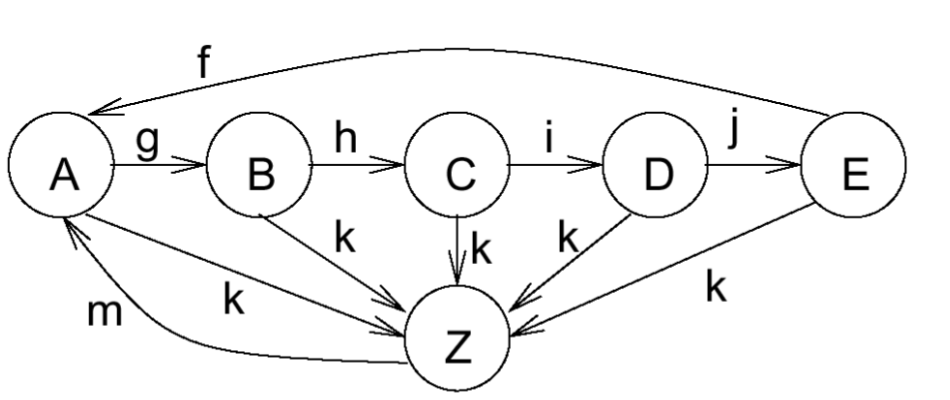
\includegraphics[width = 10cm]{images/FSM/reset_state}

\newcommand{\kreis}[1]{\unitlength1ex\begin{picture}(2.5,2.5)%
\put(0.75,0.75){\circle{3.5}}\put(0.75,0.75){\makebox(0,0){#1}}\end{picture}}

\subsection{Statecharts von Harel}
\subsubsection{Elemente der Statechart}
\begin{tabular}{ll}
$\bullet$&Anfangszustand (initial pseudo state)\\
$\diamond$& Entscheidung (choice)\\
$\bullet$& Kreuzung (junction)\\
$\times$& Terminator (terminate pseudo state)\\
\kreis{H}&flache Historie (shallow history): History-Mechanismus merkt sich
frühere Zustände\\
\kreis{H*}&tiefe Historie (deep history): Deep History-Mechanismus merkt sich
Zustände bis in die unterste Hierarchie\\
\kreis{}&Eintrittspunkt (entry point)\\
$\otimes$&Austrittspunkt (exit point)\\
\end{tabular}

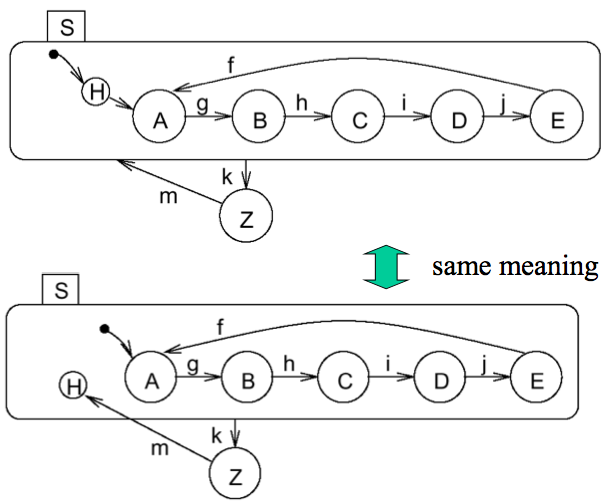
\includegraphics[scale = 0.3]{images/FSM/history_default_state_mechanism}  

\subsubsection{Definitonen}
\begin{itemize}
  \item Current states of FSMs are also called \textbf{active} states.
  \item States which are not composed of other states are called \textbf{basic
  states}.
  \item States containing other states are called \textbf{super-states}.
  \item for each basic state s, the super-states containing s are called
  \textbf{ancenstor states}.
  \item Super-states S are called \textbf{OR-super-states}, if exactly one of
  the sub-states of S is active whenever S is active.\\\\   
\end{itemize}
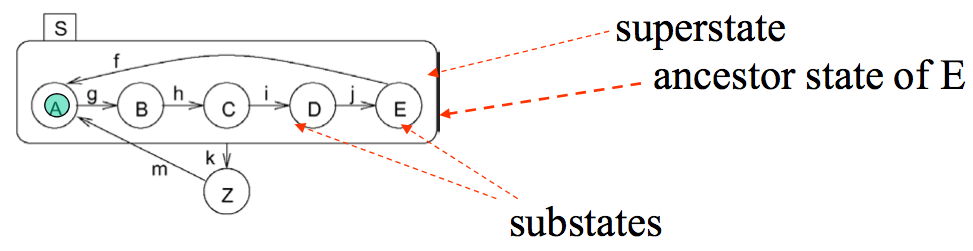
\includegraphics[scale = 0.3]{images/FSM/definition_statechart}

\subsubsection{Modellierung von Hierarchie}
\begin{itemize}
  \item Hierarchie wird mit Hilfe von Superzuständen (superstates) eingeführt.
  \item Zustände, die andere Zustände enthalten, heissen Superzustände.
  \item Zustände, die in anderen Zuständen enthalten sind, heissen Unterzustände der Superzustände.
\end{itemize}
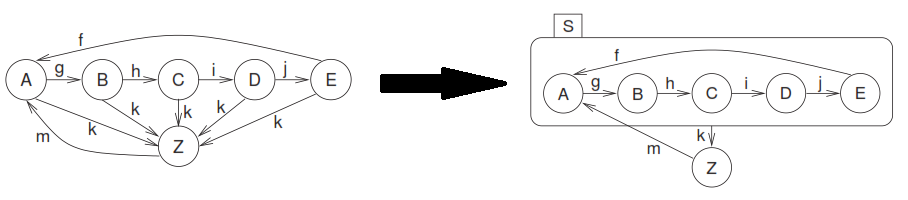
\includegraphics[width = 12cm]{images/FSM/Hierarchie}\\\\
Superzustand S beinhaltet die Zustände A, B, C, D und E. Angenommen, der Automat befindet sich in Zustand Z (wird auch als aktiven Zustand beschrieben). Wenn dann die Eingabe m am Automaten erfolgt, ist A der nächste Zustand. Wenn sich der Automat in Zustand S befindet und es gibt die Eingabe k, so ist Z der nächste Zustand, unabhängig davon, in welchem
der Unterzustände A, B, C, D oder E sich der Automat tatsächlich befindet.In diesem Beispiel sind alle in S enthaltenen Zustände nicht-hierarchische Zustände. Im Allgemeinen könnten die Unterzustände von S selbst wieder Superzustände sein, die weitere Unterzustände enthalten.
\begin{itemize}
  \item Jeder Zustand, der nicht aus anderen Zuständen besteht, heisst Basiszustand.
  \item Superzustände S heissen ODER-Superzustände, wenn das System, das S enthält, sich zu jedem Zeitpunkt lediglich in einem einzigen Unterzustand von S befinden kann, solange es sich in S befindet.
\end{itemize}
\subsubsection{History}
\subsubsection{Parallälität (Concurrency)}
\begin{itemize}
  \item AND-super-states: Die FSM ist in allen sub-states einer super-state (siehe Abbildung \ref{fig:AND_super_state})
\end{itemize}
\begin{figure}[h]
  \centering
  {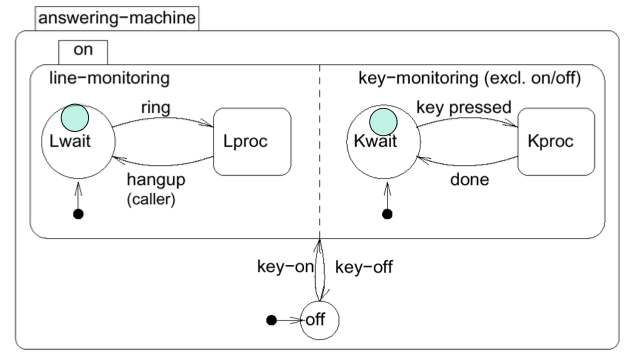
\includegraphics[scale = 0.4]{images/FSM/AND_super_state}  
  \caption{AND-super-state}
  \label{fig:AND_super_state}}
\end{figure} 

\subsubsection{Timers (nicht wait states)}
\begin{figure}[h]
  \centering
  {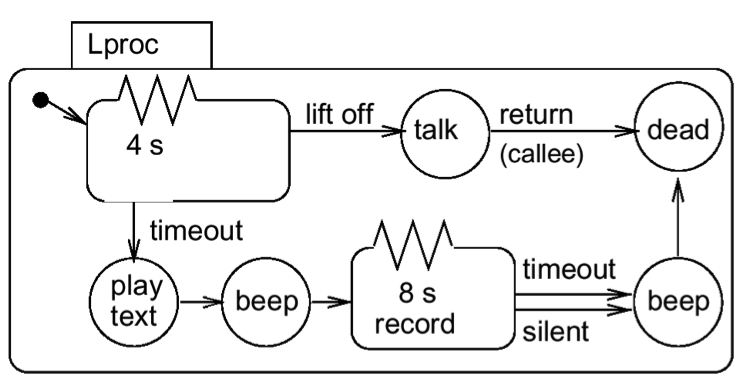
\includegraphics[scale = 0.2]{images/FSM/timer}  
  \caption{Using timers in an  answering machine}
  \label{fig:timer}}
\end{figure} 

\subsubsection{Vergleiche}
Statecharts im "`Lehrbuch der Objektmodellierung"':
\begin{itemize}
  \item LE4: pp87-95
  \item LE8: pp 197-205
  \item LE13: pp 339-348
\end{itemize}
\newpage
